\part{Technical description}
\chapter{Hardware}
\section{Introduction to CSE1}
The CS Enterprise I was initially bought in 2009, as a fully configured model boat named "Aziz" built by Model Slipway. Due to requirements for master and PhD experiments, the model was refitted by \cite{Skaatun2011}. The work performed on CS Enterprise I include, but is not limited to, dynamic positioning systems, maneuvering systems and path following, and navigation with virtual reality.

The vessel is a 1:50 scale model of a tug boat, and is fitted with two Voith Schneider propellers(VSP) astern and one bow thruster(BT). The main dimensions of the vessel are:
\begin{table}[h!]
	\caption{Main dimensions of CSE1}
	\centering
	\begin{tabular}{cc}
		\hline
		LOA & 1.105[m]\\
		B & 0.248 [m]\\
		$\Delta$ & 14.11 [kg]\\\hline
	\end{tabular}
\end{table}

\subsection{Literature}
The development of CSE1 is a product of much research from several theses, which contain complementary information on the theory applied to the system. 
\subsubsection{Journals and conferences}
\begin{itemize}
	\item LOS guidance for towing an iceberg along a straight-line path \citep{OrstenNorgrenSkjetne2014}
\end{itemize}
\subsubsection{Specialization projects and master theses}
\begin{itemize}
	\item Development of a DP system for CS Enterprise I with Voith Schneider thrusters. \citep{Skaatun2011}
	\item Development of a modularized control architecture for CS Enterprise I for path-following based on LOS and maneuvering theory \citep{Tran2013}
	\item Automatic Reliability-based Control of Iceberg Towing in Open Waters \citep{Orsten2014}
	\item Line-Of-Sight-based maneuvering control design, implementation, and experimental testing for the model ship C/S Enterprise I.\citep{Tran2014}
	\item Remote Control and Automatic Path-following for C/S Enterprise I and ROV Neptunus \citep{Sandved2015}
	\item Marine Telepresence System \citep{Valle2015}
	\item Nonlinear Adaptive Motion Control and Model-Error Analysis for Ships-Simulations and MCLab experiments \citep{bjorne2016nonlinear}
	\item Low-Cost Observer and Path-Following Adaptive Autopilot for Ships \citep{mykland2017}
\end{itemize}
\subsubsection{Other}
\begin{itemize}
	\item YouTube video \citep{Skaatun2014}
\end{itemize}

\section{Actuators}
Figure \ref{fig:position_of_actuators} illustrate the position of the actuators, and their distance from CO is given in Table \ref{tab:thruster_distance}. The BT and VSP motor speeds are controlled by an Electronic Speed Control(ESC). The ESC receive their setpoints as pulse-width modulated (PWM) signals from the cRIO digital output module. The VSP blade pitches are controlled by servos. The servos also receive their setpoint as PWM signals.

\begin{minipage}{\textwidth}
	\begin{minipage}[b]{0.49\textwidth}
		\centering
		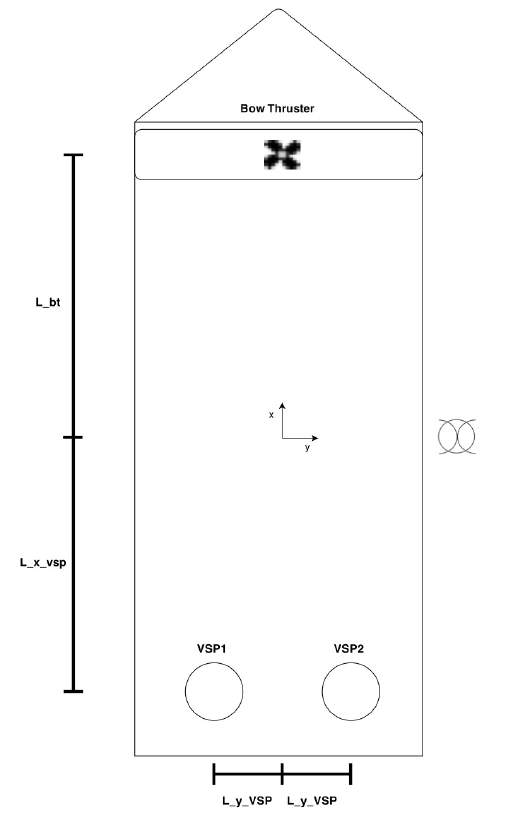
\includegraphics[width=\linewidth]{fig/actuators_overview.png}
		\captionof{figure}{Position of actuators. Adapted from \cite{Valle2015}}
		\label{fig:position_of_actuators}
	\end{minipage}
	\hfill
	\begin{minipage}[b]{0.49\textwidth}
		\centering
		\begin{tabular}{ccc}
		\hline
		\textbf{Parameter} & \textbf{Symbol} & \textbf{Value}[m]\\\hline
		x length to VSP & $L_{x,VSP}$ & -0.4574\\
		x length to BT & $L_{BT}$ & 0.3875\\
		y length to VSP & $L_{y,VSP}$ & 0.055\\\hline
		\end{tabular}
	\captionof{table}{Position of actuators}
	\label{tab:thruster_distance}
	\end{minipage}
\vspace{0.5cm}
\end{minipage}

\section{Power system}
CSE1 is powered with one 12V 12Ah battery on-board. Some of the components require different voltage, and thus some voltage converters are mounted. However, the setup works as it is, and by connecting the battery to the wires, the whole system is powered. A schematic of the power grid is illustrated in Figure \ref{fig: CSE1 power}, and Figure \ref{fig:battery_connected} show a photo of the battery mounted and connected. 
\begin{figure*}[htb!]
\centering
\begin{subfigure}{.45\linewidth}
	\centering
	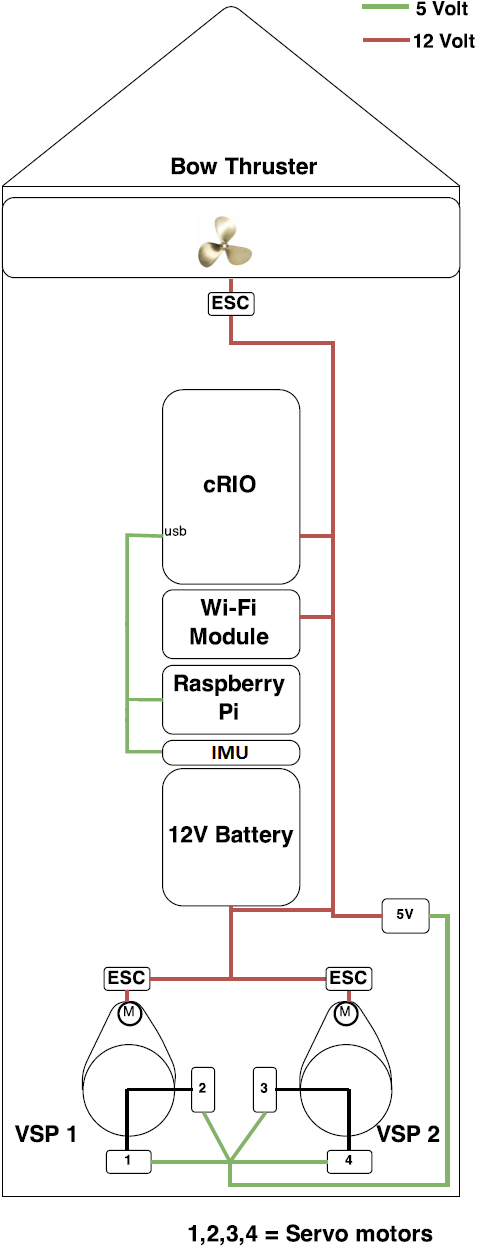
\includegraphics[height=0.4\paperheight]{fig/CSE1_power}
	\caption{CSE1 power system}
	\label{fig: CSE1 power}
\end{subfigure}
\begin{subfigure}{0.45\linewidth}
	\centering
	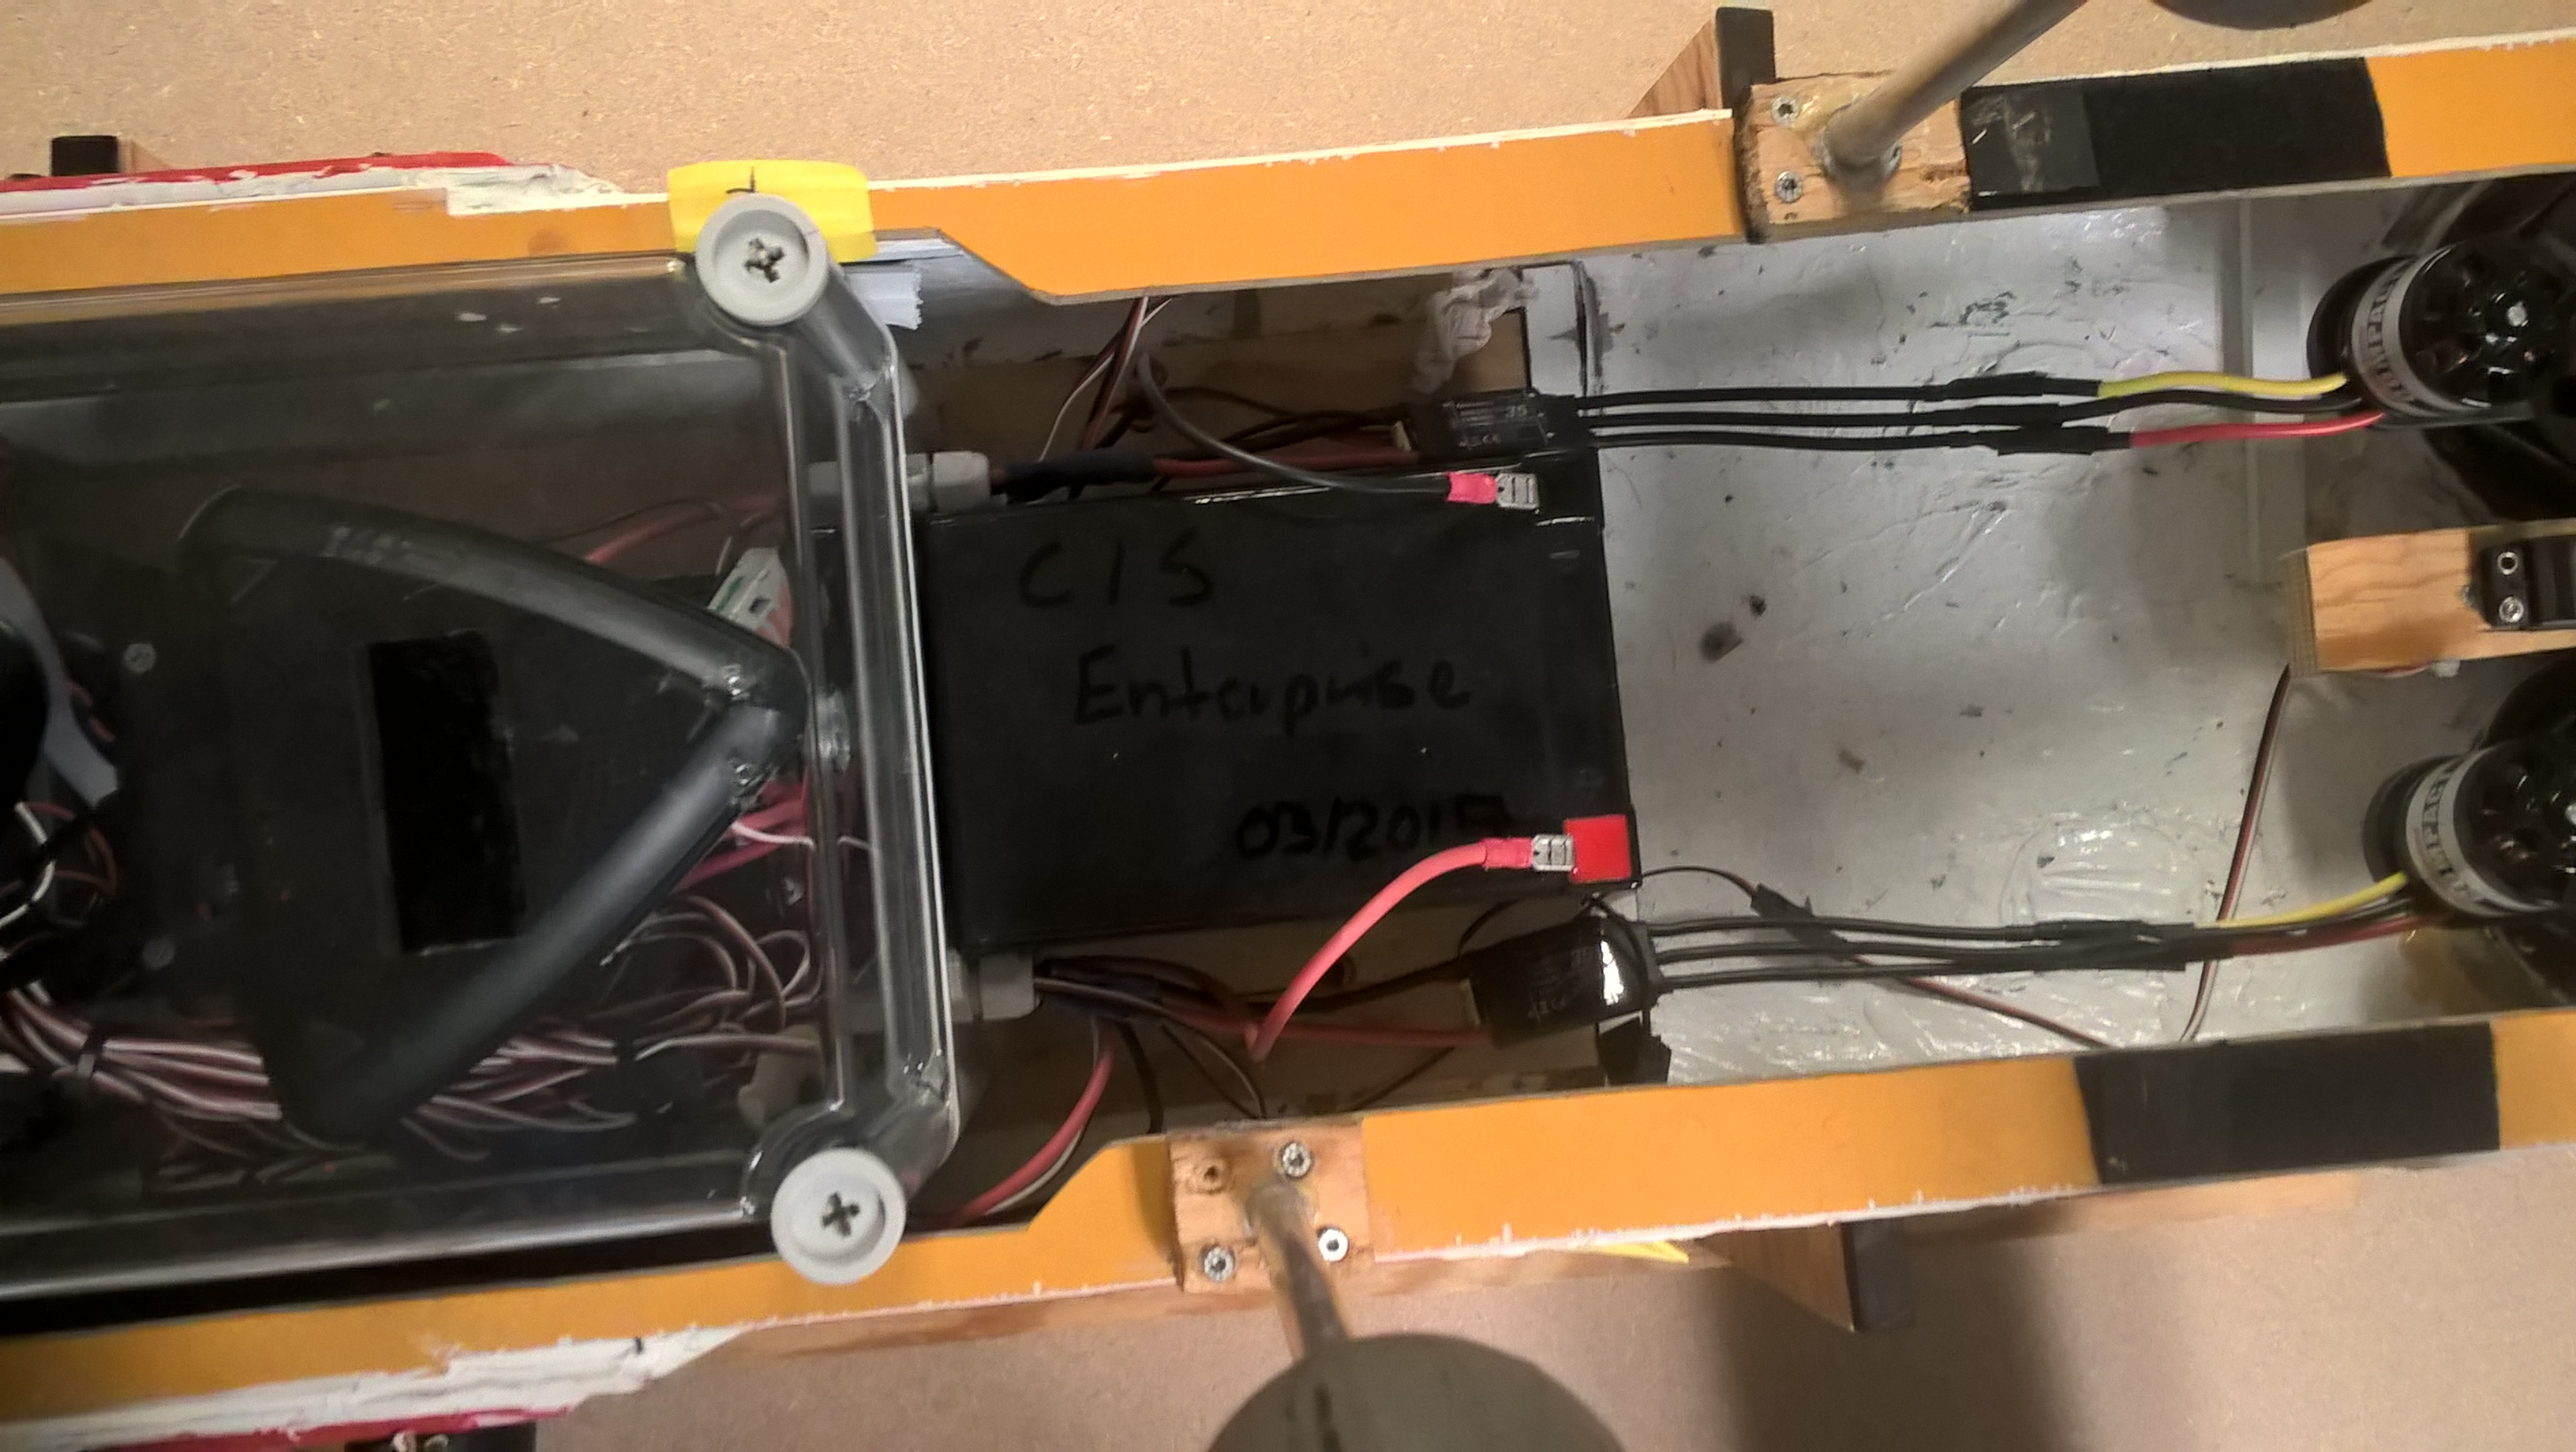
\includegraphics[width=\linewidth]{fig/battery_mounted.jpg}
	\caption{Battery mounted and connected}
	\label{fig:battery_connected}
\end{subfigure}
\caption{Battery system}
\end{figure*}

\section{IMU}
CSE1 is equipped with one Inertial Measurement Unit (IMU) from Analog Devices. The sensor mounted on-board is the ADIS16470 and includes a triaxis gyroscope and triaxis accelerometer. The sensor has built-in compensation for bias, alignment and sensitivity, and thus provides accurate measurements over a temperature range of -10 to +75 degrees Celsius. The sampling rate is set to 100 Hz. The most relevant data is presented in Table \ref{tab:IMU_specifications}, and for supplementary information the reader is referred to the data sheet \cite{adis16470}. The coordinate frame of the sensor is illustrated in Figure \ref{fig:IMU_reference_frame}, with positive directions illustrated by arrows. THe the sensor is mounted with a different orientation than the body frame, as can be seen in Figure \ref{fig:IMU_mounted}. Using the \textit{zyx}-convention, the sensor frame has an orientation relative body frame: $(\phi, \theta, \psi) = (\pi, 0, 0)$. Hence, by using the rotation matrix with these values, the measured accelerations and angular rates can be rotated to the body-frame. 
\begin{table}[htb!]\caption{IMU specifications}\label{tab:IMU_specifications}
	\centering
	\begin{tabular}{c|c|c|c|}
		\cline{2-4}
		& \textbf{Parameter} & \textbf{Typical value} & \textbf{Unit}\\ \cline{1-4}
		\multicolumn{1}{|c|}{\multirow{5}{*}{\textbf{Gyroscopes}}} & Dynamic range & $\pm 2000$ & \degree/sec\\ 
		\multicolumn{1}{|c|}{} & Sensitivity & 10 & LSB/\degree/sec\\ 
		\multicolumn{1}{|c|}{} & Bias stability, $\sigma$ & 8 & \degree/hr\\ 
		\multicolumn{1}{|c|}{} & Angular random walk & 0.34 & \degree/$\sqrt{hr}$\\ 
		\multicolumn{1}{|c|}{} & Output noise & 0.17 & \degree/sec rms\\ \cline{1-4}
		
		\multicolumn{1}{|c|}{\multirow{5}{*}{\textbf{Accelerometers}}} & Dynamic range & $\pm 40$ & g\\ 
		\multicolumn{1}{|c|}{} & Sensitivity & 800 & LSB/g\\ 
		\multicolumn{1}{|c|}{} & Bias stability, $\sigma$ & 0.013 & mg\\ 
		\multicolumn{1}{|c|}{} & Velocity random walk & 0.037 & m/sec/$\sqrt{hr}$\\ 
		\multicolumn{1}{|c|}{} & Output noise & 2.3 & mg rms\\ \cline{1-4}
		
		\multicolumn{1}{|c|}{\multirow{1}{*}{\textbf{Power supply}}} & Operating voltage& $3.3 \pm 0.3$ & V\\ \cline{1-4}
	\end{tabular}
\end{table}
\begin{figure}[htb!]
	\centering
	\begin{subfigure}{0.45\linewidth}
		\centering
		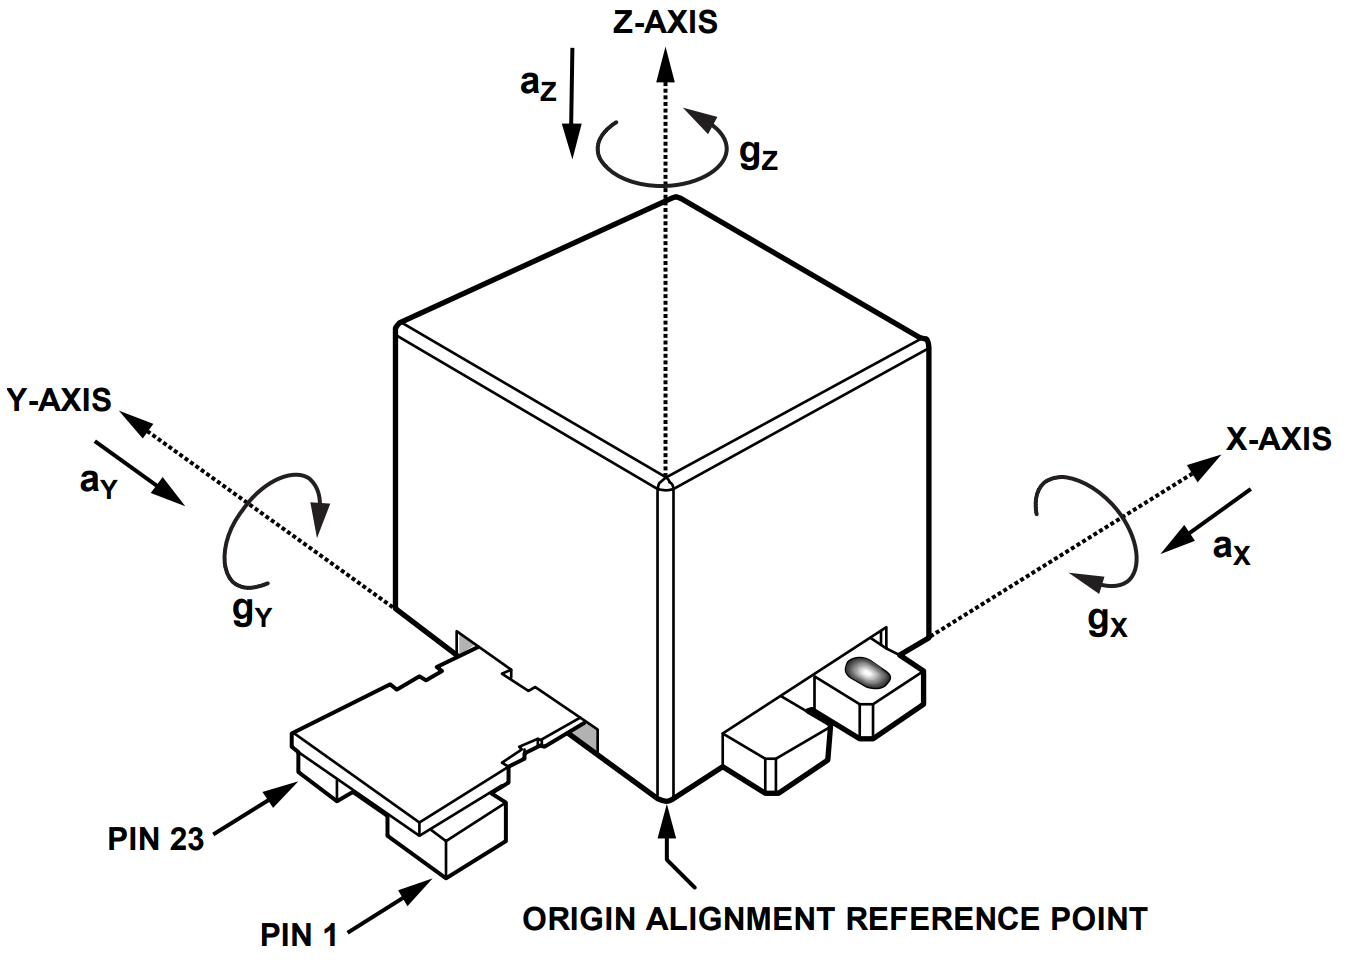
\includegraphics[width=1\linewidth]{fig/IMU_reference_frame.png}
		\caption{IMU reference frame from manufacturer}
		\label{fig:IMU_reference_frame}
	\end{subfigure}
	\begin{subfigure}{0.45\linewidth}
		\centering
		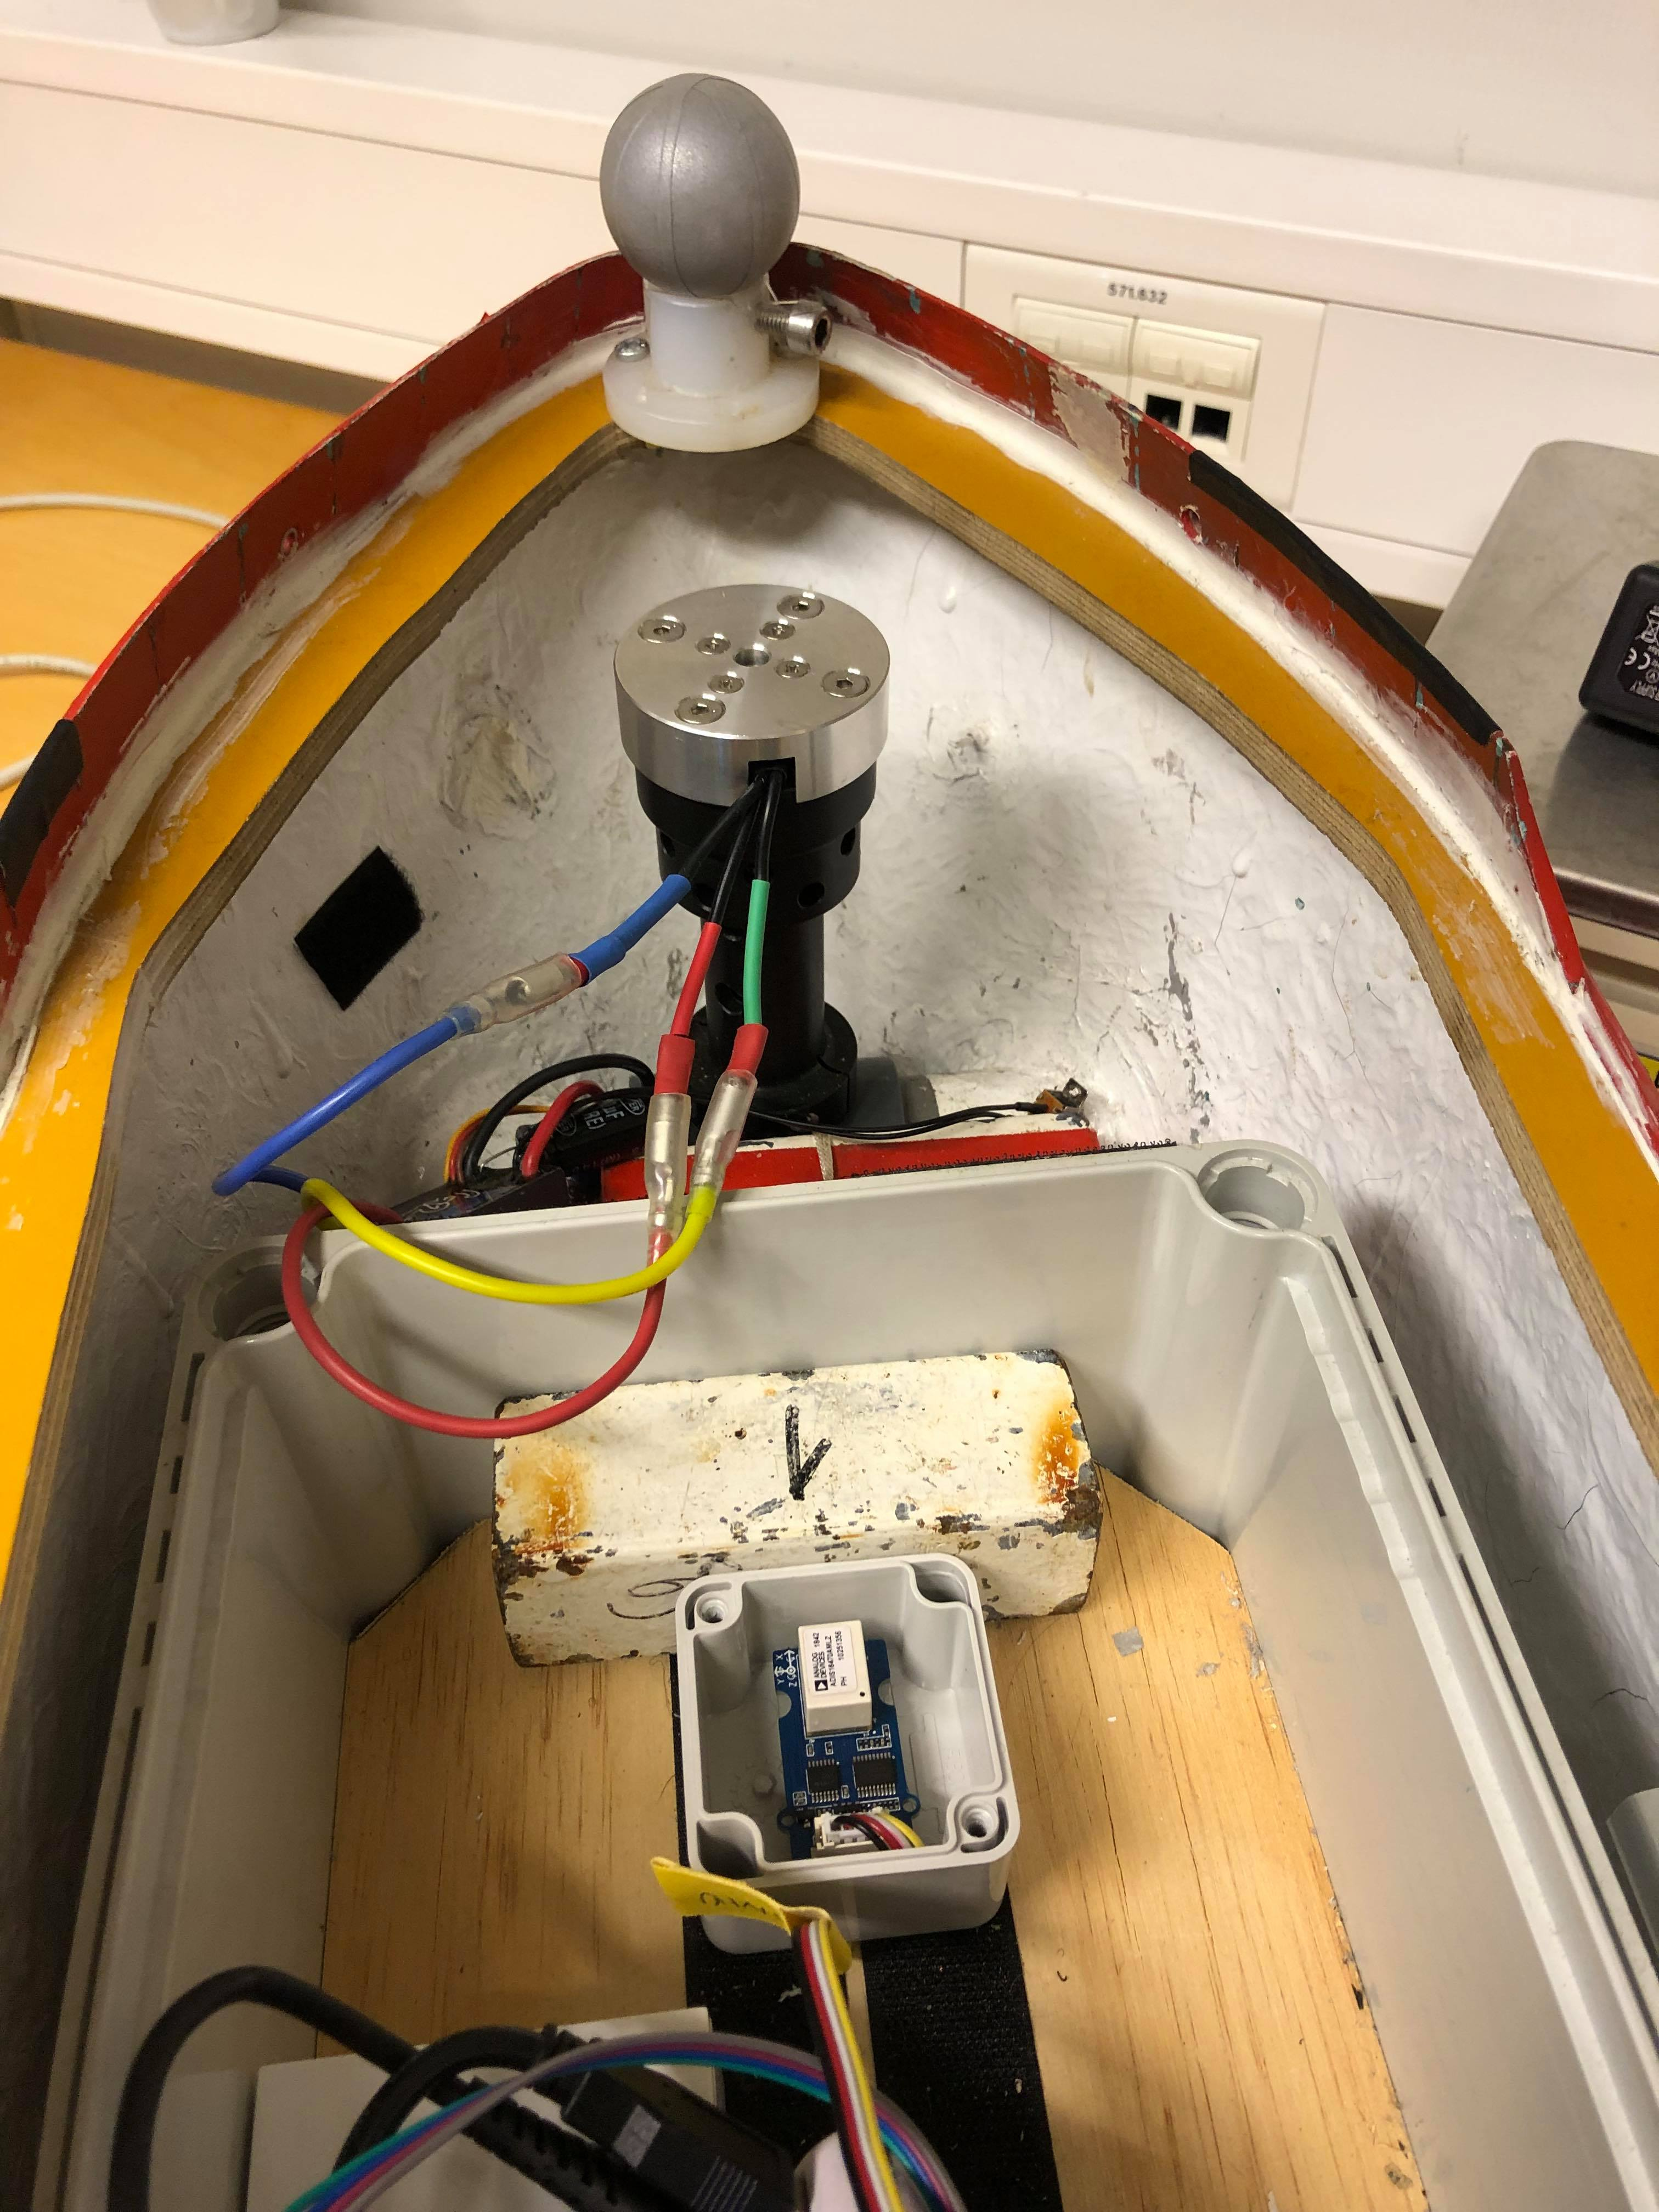
\includegraphics[width=0.9\linewidth]{fig/IMU_mounted.jpg}
		\caption{IMU mounted in the vessel}
		\label{fig:IMU_mounted}
	\end{subfigure}
\caption{Inertial Measurement Unit in CSE1}
\end{figure}

\section{Control system}
The on-board control system consists of the following parts:
\begin{itemize}
	% \item a National Instruments compact reconfigurable input/output (cRIO)
	% embedded controller
	\item a Raspberry Pi 4 (RPi) single-board computer
	\item three electronic speed controllers (ESC)
	\item four servos
\end{itemize}
% \subsection{cRIO}
% The model on-board is the cRIO-9024, and it is connected to 4 FPGA modules for analogue and digital I/O:
% \begin{itemize}
% 	\item NI-9215, used for analog input such as measuring voltage
% 	\item NI-9263, used for reading IMU measurements
% 	\item NI-9401, not used
% 	\item NI-9474, used for sending pwm signal
% \end{itemize}
\subsection{RPi}

The Raspberry Pi provides communication 
with the DS4 controller, the servos and the electronic speed controllers.. It works as an embedded system, and once powered it will start searching for the wireless controller. When connection is established, it will continuously send signals to the servos and ESC based on operation mode. To successfully connect the sixaxis controller to the RPi, wait for the Bluetooth dongle to start blinking before pressing the PS-button on the controller. 

\subsection{ESC}
The ESC's are controlled with PWM signals, based on PWM tick signals. Table \ref{tab:pwm_spec} describe the setup for all ESC's on-board CSE1, and Table \ref{tab:pwm_range} gives the pwm signal range for each ESC.
\begin{table}[h!]
	\centering
	\caption{PWM specification for ESC}
	\label{tab:pwm_spec}
	\begin{tabular}{cccc}
		\hline
		\textbf{Initial value} & \textbf{Scaling} & \textbf{Offset} & \textbf{PWM period} [Ticks] \\ \hline
		0 & 100 & 0 & 800.000\\ \hline
	\end{tabular}
\end{table}

\begin{table}[h!]
	\centering
	\caption{PWM ranges for ESC}
	\label{tab:pwm_range}
	\begin{tabular}{cccc}
		\hline
		& \textbf{ESC\_BT}[\%] & \textbf{ESC\_VSP1}[\%] & \textbf{ESC\_VSP2}[\%]\\ \hline
		\textbf{min} & 7.00 & 3.12 & 3.12\\
		\textbf{neutral} & 7.55 & 5.01 & 5.01\\
		\textbf{max} & 8.10 & 6.90 & 6.90\\ \hline
	\end{tabular}
\end{table}

\chapter{Software}
\section{Introduction}

The control system of CSE1 is built around a framework called Robot Operating System. ROS consists of tools, libraries, and conventions that help in building robot applications. This chapter gives a description of vessels software hierarchy. Note that most of this software is ready to use, and alterations in the software described here should not be necessary, unless specified.


\section{Driver setup}

\subsection{Actuator drivers}
To activate the actuators on the vessel, first SSH to the onboard RPi 4 and launch nodelet manager and the CSE actuator driver:
\begin{lstlisting}[language=bash,basicstyle=\mlttfamily, breaklines=true]
  $ rosrun nodelet nodelet manager __name:=nodelet_manager
  $ rosrun nodelet nodelet load cse_actuator_driver/cse_actuator_driver_nodelet  
  nodelet_manager __name:=cse_actuator_driver
\end{lstlisting}
You should hear a beeping sound if the nodes are succesfully run. 
\subsection{Qualisys drivers}
Next is to launch the Qualisys drivers. These are written in ROS2 rather than ROS1 and  must be activated from the ROS2 workspace it is installed to, either from the onboard RPi, or from another computer connected to the MCLab network: 
\begin{lstlisting}[language=bash,basicstyle=\mlttfamily, breaklines=true]
  $ ros2 run ros2_qualisys_driver qualisys_driver_exe 
  --ros-args --params-file src/ros2_qualisys_driver/params/params.yaml
  $ ros2 lifecycle set /qualisys_driver configure
  $ ros2 lifecycle set /qualisys_driver activate
\end{lstlisting}

To source ROS2 or ROS1 in the workspace, use:

\begin{lstlisting}[language=bash,basicstyle=\mlttfamily, breaklines=true]
  $ . /opt/ros/$ROS_DISTRO/setup.zsh
\end{lstlisting}\footnote{\$ROS\_DISTRO may vary, but is most likely \textbf{foxy} for ROS2 and \textbf{noetic} for ROS1}
Then you have to run the ROS2 bridge that allows the qualisys driver to properly communicate with the ROS1 drivers. 

\begin{lstlisting}[language=bash,basicstyle=\mlttfamily, breaklines=true]
  $ ros2 run ros1_bridge dynamic_bridge --bridge-all-2to1-topics
\end{lstlisting}

Since the \textbf{roscore} is likely running on the raspberry, you will also have to export the IP of the Pi and Rosmaster: 

\begin{lstlisting}[language=bash,basicstyle=\mlttfamily, breaklines=true]
  $ export ROS_MASTER_URI=http://192.168.0.171:11311 
  $ export ROS_IP=192.168.0.104
\end{lstlisting}

\subsection{IMU-drivers}

To read the data from the IMU, their drivers first have to be read. These are written in C++, but are compatible with a ROS-system written in Python or Matlab. Put the \lstinline{imu_driver} package inside your workspace \textbf{src}-directory and run \lstinline{catkin_make}. After the package is built, first source the bash file and then simply run the package.

\begin{lstlisting}[language=bash,basicstyle=\mlttfamily, breaklines=true]
  $ source devel/setup.bash
  $ rosrun imu_driver imu_node
\end{lstlisting}

The driver publishes the measurements to the topic \textbf{/imu}. 


\section{ROS with Python}

The python based software for CSEI consists of 5 premade packages; \textbf{controller}, \textbf{observer}, \textbf{messages}, \textbf{gain\_server}, \textbf{simulator} and \textbf{tf\_publisher}. This section will document each package. 

\subsection{Prerequisites and recommended software}

\textbf{Required:}
\begin{itemize}
    \item Python 3.8.3 +
\end{itemize}
\textbf{Recommended:}
\begin{itemize}
    \item Visual Studio Code with the \textbf{Remote SSH} extension. This enables you to SSH directly in to raspberry via VS Code, allowing you to edit files on the pi in the text-editor.
    \item A computer running linux. This is not required as most software will run on the Raspberry Pi, but can be beneficial for testing and visualizing.
\end{itemize}
\subsection{Sourcing your ROS-distribution}

Before you do anything with ROS, you need to source the installation. On the RP this is done automatically, but in case you are working on your own computer the following steps are necessary: 

\begin{lstlisting}[language=bash,basicstyle=\mlttfamily, breaklines=true]
  $ source /opt/ros/DISTRIBUTION/setup.bash
\end{lstlisting}

\subsection{Building a catkin workspace}

To run ROS-packages we must first define a worspace for them on the Pi. SSH onto the pi and run 

\begin{lstlisting}[language=bash,basicstyle=\mlttfamily, breaklines=true]
  $ mkdir -p workspace/src; cd workspace
  $ catkin_make
\end{lstlisting}

This should build your catkin workspace, and leave you with three sub-directories; \textbf{build}, \textbf{devel} and \textbf{src}. All ROS-packeges are placed in the \textbf{src}-directory. Everytime you add a package to the workspace, rebuild it using \lstinline{catkin_make}.

\subsection{Running packages}

To run your packages, first make sure you have sourced the \lstinline{setup.bash} file:

\begin{lstlisting}[language=bash,basicstyle=\mlttfamily, breaklines=true]
  $ source devel/setup.bash
\end{lstlisting}

Then, to run the package use

\begin{lstlisting}[language=bash,basicstyle=\mlttfamily, breaklines=true]
  $ rosrun <package-name> <node-script>.py
\end{lstlisting}

where <package-name> is the name of the package you want to run, e.g "controller", and the <node-script>.py is the python script that initialisez the rosnode, e.g "ctrl\_node.py". 


\subsection{The controller package}
The first ROS-package is the \textit{controller}-package. It contains relevant tools and scripts to build guidance systems, regulators and thrust-allocation. In total, the package contains six scripts.

\subsubsection{math\_tools.py}
As the name implies, \lstinline{math_tools.py} contains functions related to math-operations. For example computing Rotation-matrices, converting quaternions, etc. The user should add to this file according to their needs, and import the functions in other relevant files. 

\subsubsection{lib.py}
\lstinline{lib.py} contains the tools related to extracting and publishing the data from the different ROS-nodes in the system, as well as the functions for initializing and destroying the controller node. The tools are class-based, with one object for every relevant parameter in the control system. Each object contains methods for publishing new information, retrieving information from other nodes. In total there are five classes:
\begin{itemize}
    \item \textbf{PS4}: This object subscribes to the topic \textbf{/joy} and is automatically updated with inputs from the DualShock4 controller. Each button input is mapped to a corresponding variable, which can be called by in the pattern of \lstinline{<object.variable>}. I.e \lstinline{ps4.R2} returns the current signal from the R2 button.
    \item \textbf{UVector}:
    The UVector object publishes the inputs to the vessel actuators. After computing $u$, call the function \lstinline{UVector.publish(u)} to publish the array.
    \item \textbf{Observer\_Converser}:
    The Observer\_Converser subscribes to the topic \textbf{/CSEI/observer} and automatically updates every time a observer estimations are published. The estimates can be called by 
    \begin{lstlisting}[language=python,basicstyle=\mlttfamily, breaklines=true]
    eta_hat, nu_hat, bias_hat = observer.get_observer_data()
    \end{lstlisting}
    \item \textbf{Reference\_Converser}:
    Similar to the observer\_converser, except that it subscribes to the /CSEI/ref topic and contains methods for publishing as well. References are extracted and published by
     \begin{lstlisting}[language=python,basicstyle=\mlttfamily, breaklines=true]
    eta_d, nu_d, nu_d_dot = reference.get_ref() # Call reference
    refrence.publish_ref(eta_d, nu_d, nu_d_dot) # Publish new reference
    \end{lstlisting}
    \item \textbf{Controller\_Gains}:
    The Controller\_Gains object is updated every time the user re-configures the controller-gains. To extract the new gains, call:
     \begin{lstlisting}[language=python,basicstyle=\mlttfamily, breaklines=true]
    Kp, Kd, Ki, mu, Uref = gains.get_data()
    \end{lstlisting}
\end{itemize}

All objects are declared in the script, and can be imported in custom scripts at the users behest: 
    \begin{lstlisting}[language=python,basicstyle=\mlttfamily, breaklines=true]
    from lib import ps4, Uvector, observer, reference, Gains
    \end{lstlisting}
    
\subsubsection{ctrl\_joy.py}

\lstinline{ctrl_joy.py} is the default control-software for the CSE1. It enables manual control of the vessel thrusters  using the DS4 controller.

% \subsubsubsection{Bow thruster}

% The bow tunnel thruster is controlled by the L2 and R2 sticks. Both stick provide an output in the intervall $[0, 1]$. The thruster input  

% \begin{equation}
%     u_1 = -\frac{L2 - R2}{2}
% \end{equation}

% maps to the intervall $u_1 \in [-1, 1]$ with positiv direction towards starboard.

% \subsubsubsection{Voith Schneider Propellers}

% The left and right joysticks, respectively, give the VSP deflections, $u_1$ and $u_2$, and angles, $\alpha_1$ and $\alpha_2$. The joystick coordinates PosX and PosY axes point right and down, as seen in Figure \ref{fig:sixaxis coordinate system}. The deflection is 


% \begin{equation}
%     u_i = min\left(\sqrt{(posX)^2 + (posY)^2}, 1  \right)
% \end{equation}

% where the $min(\cdot)$ ensures the deflection is constrained on $u_i \in [0,1]$. The angle is 

% \begin{equation}
%     \alpha_i = \arctan2(PosX, -PosY)
% \end{equation}


\subsubsection{ctrl\_stud.py}

This is a skeleton file, where custom control systems are to be implemented. It contains a \lstinline{loop()} function, which operates similar to a main function. All function-calls should be handled inside this function.


\subsubsection{ctrl\_node.py/ctrl\_joy\_node.py}
These are the scripts that initialize and launch the ROS nodes, and are generally not meant to be reconfigured. They initialize the nodes at 100 Hz and call the \lstinline{loop()}-function from either \lstinline{ctrl_joy} or \lstinline{ctrl_stud}.

To manually run the package using either \lstinline{ctrl_joy} or \lstinline{ctrl_stud} use:

 \begin{lstlisting}[language=python,basicstyle=\mlttfamily, breaklines=true]
 rosrun controller ctrl_joy_node.py # For ctrl_joy
 rosrun controller ctrl_node        # For ctrl_stud
 \end{lstlisting}

\subsection{The observer package}

The observer package handles everything related to observer implementation, and is very similar in structure to the controller package. It has a total of four scripts, one being a \lstinline{math_tools.py} identical to the one in controller.

\subsubsection{lib.py}

\lstinline{lib.py} contains the tools related extracting and publishing the data from the different ROS-nodes in the system, as well as the functions for initializing and destroying the observer node. Like with the controller package, The tools are class-based, with one object for every relevant parameter in the control system. Each object contains methods for publishing new information, retrieving information from other nodes. The observer package utilizes the same UVector-class as the controller, along with a couple new.

\begin{itemize}
    \item \lstinline{qualisys}: This object subscribes to the \textbf{/qualisys} topic, and retrieves the position the system captures of the vessel. To retrive the data call on the method: 
    
    \begin{lstlisting}[language=python,basicstyle=\mlttfamily, breaklines=true]
    eta_hat = qualisys.getQualisysOdometry()
    \end{lstlisting}
    
    \item \lstinline{Observer_Converser}: Identical to the object described in the controller package. Also contains methods for publishing the observer data: 
     \begin{lstlisting}[language=python,basicstyle=\mlttfamily, breaklines=true]
    eta_hat, nu_hat, bias_hat = observer.get_data()           # Return newest estimate
    observer.publish_observer_data(eta_hat, nu_hat, bias_hat) # Publish computed estimate
    \end{lstlisting}
    
    \item \lstinline{Observer_Gains}
    Retrieves the injection gains for the observer in a similar manner as Controller\_Gains. 
    \begin{lstlisting}[language=python,basicstyle=\mlttfamily, breaklines=true]
    L1, L2, L3 = Gains.get_observer_gains()           # NB! These are np.arrays with n=3 
    \end{lstlisting}
\end{itemize}

\subsubsection{obs\_stud.py}
Skeleton file for implementation of observer. All user-defined functions must be called in the right order in the \lstinline{loop()} function. 

\subsubsection{obs\_node.py}
Initializes the observer node

\subsection{The gain\_server package}

gain\_server utilizes another ROS-package called dynamic reconfiguration. This enables the user to reconfigure parameters in a ROS-node during runtime. For the Enterprise, this allows for dynamic tuning of the control-system gains. To run the package: 

\begin{lstlisting}[language=bash,basicstyle=\mlttfamily, breaklines=true]
  $ rosrun gain_server server.py
\end{lstlisting}

To tune parameters from the command-line use: 

\begin{lstlisting}[language=bash,basicstyle=\mlttfamily, breaklines=true]
  $ rosrun dynamic_reconfigure dynparam set gain_server parameter_name value
\end{lstlisting}

Alternatively, it is possible to create a .yaml file with all parameters which can be edited and subsequently uploaded to the node. To create the file, and load the new parameters run: 

\begin{lstlisting}[language=bash,basicstyle=\mlttfamily, breaklines=true]
  $ rosrun dynamic_reconfigure dynparam dump gain_server gains.yaml
  $ rosrun dynamic_reconfigure dynparam load gain_server gains.yaml
\end{lstlisting}

\subsubsection{Parameters}

Currently, the package supports a fixed set of parameters. These are observer injection gains $L1, L2, L3$ as well as the controller gains $Kp, Kd, Ki$, $\mu$ and $Uref$. If other parameters are needed these must be added to the \textbf{gains.cfg} file in the cfg-directory. 

\subsubsection{GUI-Setup}

If using the GUI-laptop in the MC-Lab, the gains can be tuned via a GUI. To open it, run the following command from the terminal: 
\begin{lstlisting}[language=bash,basicstyle=\mlttfamily, breaklines=true]
  $ rosrun rqt_gui rqt_gui -s reconfigure
\end{lstlisting}

\subsection{Launch files}

Instead of manually activating each node, you can initialize several at the same time using a launch file. These can be found in the folder \textbf{launch} in each package. 

\begin{lstlisting}[language=bash,basicstyle=\mlttfamily, breaklines=true]
  $ roslaunch package_name launch_file
\end{lstlisting}

\subsection{Usefull ROS-commands}

The following command-line tools are usefull when running a ros system: 

\begin{enumerate}
    \item \begin{lstlisting}[language=bash,basicstyle=\mlttfamily, breaklines=true]
  $ rostopic list \end{lstlisting} - Shows a list of all ROS-topics 
  
    \item \begin{lstlisting}[language=bash,basicstyle=\mlttfamily, breaklines=true]
  $ rosnode list\end{lstlisting} -
    Shows a list of all active ROS-nodes
     \item \begin{lstlisting}[language=bash,basicstyle=\mlttfamily, breaklines=true]
  $ rostopic echo topic\end{lstlisting} - Prints the messages and data sent to each topic to the command-line window
\end{enumerate}


